\section{Ejercicio 4}

\subsection{Introducción}
\noindent El objetivo de este ejercicio es resolver nuevamente el problema de MCS, pero esta vez con una heurística constructiva golosa, ya que suponemos que resolver el problema de forma exacta no se puede hacer en tiempo polinomial, pero sí podemos implementar un algoritmo heurístico que se ejecute eficientemente (tiempo polinomial) aunque no garantice la solución óptima.\\
La heurística constructiva golosa es un algoritmo que va armando la solución tomando en cada paso la mejor elección a nivel local de un conjunto de elecciones posibles, es decir, para cada paso, tomar la decisión que sea la más conveniente en ese momento.\\
Esto puede generar que la solución no sea la óptima real ya que ésta última podría requerir mirar soluciones que no sean las óptimas en el momento pero que luego llevarán a la mejor solución posible. 

\subsection{Heurística}
\noindent El algoritmo recibe dos grafos y se quiere hallar al máximo subgrafo común entre ellos. Sea $G1$ el que tiene la menor cantidad de nodos y $G2$ el otro. Si ambos tienen igual cantidad de nodos es indistinto cual es $G1$ y cual es $G2$.\\
Sea el vector mapeo, igual al desarrollado en el ejercicio 2. Dado un mapeo, se busca cuál es el conjunto de aristas que tienen en común ambos grafos renombrando cada nodo $i$ de $G1$ como $mapeo[i]$, es decir, el nodo que antes era el nodo $i$ ahora se llamará $mapeo[i]$.\\
Para este ejercicio la heurística que se utilizará es la que mapea los nodos de forma ordenada por grados. Sea nodosPorGrados un vector que ordena los nodos de un grafo según sus grados de mayor a menor. Lo que queremos hallar es el mapeo que cumple que el nodo $i$ $\in$ $G1$ está mapeado con el nodo $j$ $\in$ $G2$ sí y sólo sí el nodo $i$ y el nodo $j$ ocupan la misma posición en el vector nodosPorGrados para cada uno de los grafos.\\

\noindent Esta heurística es válida ya que mapear ordenadamente por grados hace que, en muchos casos, la cantidad de aristas que puede ser tomada en cuenta sea la máxima posible. Si se mapea el que tiene menor grado con el de mayor grado del otro grafo lo que puede pasar es que, por ejemplo, quede uno de grado cero con uno de grado muy alto, entonces todas las aristas incidentes la de mayor grado no pueden ser tenidas en cuenta para el calculo del máximo común subgrafo. Lo que puede pasar es que por más que se mapee de esta manera, las conexiones entre los nodos queden totalmente diferentes entre los grafos. Por ejemplo, sea $G1$ el grafo $Cn$ y $G2$ un grafo compuesto por $k$ componentes conexas en donde cada una de ellas es un grafo estrella con un nodo de grado mayor o igual a 2. Supongamos que la cantidad de nodos de $Cn$ es menor que $k$. $Cn$ tiene todos nodos de grado 2, entonces a cada nodo de $Cn$ se lo mapeará con un nodo del centro de las estrellas generando así que no haya ninguna arista en común para este mapeo.\\
%supongamos que el grafo que se tiene es un conjunto de grafos estrella y el otro grafo es un ciclo (Cn). Luego el Cn tiene todos nodos de grado 2 pero el conjunto de estrella tiene tantos nodos como subgrafos estrellas haya con grados mayores o iguales a dos. Entonces si la cantidad de nodos de Cn es menor que la cantidad de componentes conexas del otro, a cada nodo de Cn se lo mapeará con un nodo del centro de las estrellas generando así que no haya ninguna arista en común para este mapeo.
\begin{figure}[H]

\hspace*{\fill} 
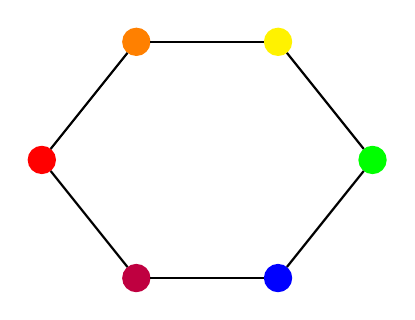
\begin{tikzpicture}[scale= 0.6]
\node[draw,circle,thick,fill,red](0) at (1,0){}; \\
 \node[draw,circle,thick,fill,orange](1) at (3,2.5){}; \\
 \node[draw,circle,thick,fill,yellow](2) at (6,2.5){}; \\
 \node[draw,circle,thick,fill,green](3) at (8,0){}; \\
 \node[draw,circle,thick,fill,blue](4) at (6,-2.5){}; \\
 \node[draw,circle,thick,fill,purple](5) at (3,-2.5){}; \\

% \draw [thick,->] (a) to [out=120,in=180] (b);
 \draw [thick] (0) -- (1);
 \draw [thick] (1) -- (2);
 \draw [thick] (2) -- (3);
 \draw [thick] (3) -- (4);
 \draw [thick] (4) -- (5);
 \draw [thick] (0) -- (5);
\end{tikzpicture}
\hspace{\fill} 
\caption{$G1=C_{6}$}
\end{figure}

\begin{figure}[H]

%\hspace*{\fill} 
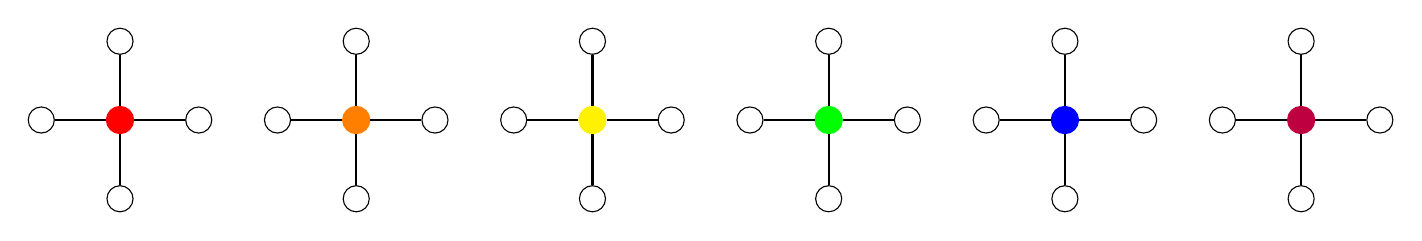
\begin{tikzpicture}[scale= 0.5]
 \node[draw,circle,thick,fill,red](0) at (0,0){}; \\
 \node[draw,circle](1) at (2,0){}; \\
 \node[draw,circle](2) at (0,2){}; \\
 \node[draw,circle](3) at (-2,0){}; \\
 \node[draw,circle](4) at (0,-2){}; \\

 \node[draw,circle,thick,fill,orange](5) at (6,0){}; \\
 \node[draw,circle](6) at (8,0){}; \\
 \node[draw,circle](7) at (6,2){}; \\
 \node[draw,circle](8) at (6,-2){}; \\
 \node[draw,circle](9) at (4,0){}; \\
 
 \node[draw,circle,thick,fill,yellow](10) at (12,0){}; \\
 \node[draw,circle](11) at (14,0){}; \\
 \node[draw,circle](12) at (12,2){}; \\
 \node[draw,circle](13) at (12,-2){}; \\
 \node[draw,circle](14) at (10,0){}; \\
 
 \node[draw,circle,thick,fill,green](15) at (18,0){}; \\
 \node[draw,circle](16) at (20,0){}; \\
 \node[draw,circle](17) at (18,2){}; \\
 \node[draw,circle](18) at (18,-2){}; \\
 \node[draw,circle](19) at (16,0){}; \\
 
 \node[draw,circle,thick,fill,blue](20) at (24,0){}; \\
 \node[draw,circle](21) at (26,0){}; \\
 \node[draw,circle](22) at (24,2){}; \\
 \node[draw,circle](23) at (24,-2){}; \\
 \node[draw,circle](24) at (22,0){}; \\
 
 \node[draw,circle,thick,fill,purple](25) at (30,0){}; \\
 \node[draw,circle](26) at (32,0){}; \\
 \node[draw,circle](27) at (30,2){}; \\
 \node[draw,circle](28) at (30,-2){}; \\
 \node[draw,circle](29) at (28,0){}; \\

% \draw [thick,->] (a) to [out=120,in=180] (b);
 \draw [thick] (0) -- (1);
 \draw [thick] (0) -- (2);
 \draw [thick] (0) -- (3);
 \draw [thick] (0) -- (4);
 
 \draw [thick] (5) -- (6);
 \draw [thick] (5) -- (7);
 \draw [thick] (5) -- (8);
 \draw [thick] (5) -- (9);
 
 \draw [thick] (10) -- (11);
 \draw [thick] (10) -- (12);
 \draw [thick] (10) -- (13);
 \draw [thick] (10) -- (14);

 \draw [thick] (15) -- (16);
 \draw [thick] (15) -- (17);
 \draw [thick] (15) -- (18);
 \draw [thick] (15) -- (19);
 
 \draw [thick] (20) -- (21);
 \draw [thick] (20) -- (22);
 \draw [thick] (20) -- (23);
 \draw [thick] (20) -- (24);
 
 \draw [thick] (25) -- (26);
 \draw [thick] (25) -- (27);
 \draw [thick] (25) -- (28);
 \draw [thick] (25) -- (29);


\end{tikzpicture}
%\hspace{\fill} 
\caption{$G2$}
\end{figure}

\noindent En las figuras se muestra en colores el mapeo que se genera con la heurística golosa. Por ejemplo, el nodo rojo en $G1$ se mapea con el nodo rojo en $G2$. Este mapeo genera la siguiente respuesta: 

\begin{figure}[H]

\hspace*{\fill} 
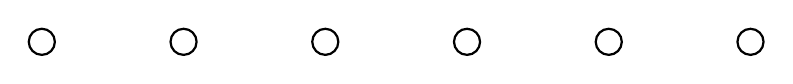
\begin{tikzpicture}[scale= 0.6]
\node[draw,circle,thick](0) at (0,0){}; \\
 \node[draw,circle,thick](1) at (3,0){}; \\
 \node[draw,circle,thick](2) at (6,0){}; \\
 \node[draw,circle,thick](3) at (9,0){}; \\
 \node[draw,circle,thick](4) at (12,0){}; \\
 \node[draw,circle,thick](5) at (15,0){}; \\
\end{tikzpicture}
\hspace{\fill} 
\caption{Grafo solución según heurística golosa}
\end{figure}

\noindent Pero la solución real es la siguiente: 
\begin{figure}[H]

\hspace*{\fill} 
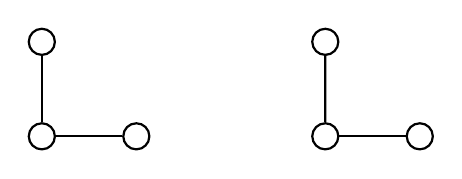
\begin{tikzpicture}[scale= 0.6]
\node[draw,circle,thick](0) at (0,0){}; \\
 \node[draw,circle,thick](1) at (0,2){}; \\
 \node[draw,circle,thick](2) at (2,0){}; \\
 \node[draw,circle,thick](3) at (6,0){}; \\
 \node[draw,circle,thick](4) at (6,2){}; \\
 \node[draw,circle,thick](5) at (8,0){}; \\

% \draw [thick,->] (a) to [out=120,in=180] (b);
 \draw [thick] (0) -- (1);
 \draw [thick] (0) -- (2);
 \draw [thick] (3) -- (4);
 \draw [thick] (3) -- (5);
\end{tikzpicture}
\hspace{\fill} 
\caption{Grafo solución}
\end{figure}


\subsection{Implementación}

El algoritmo se comporta de la siguiente manera:
\begin{itemize}
\item Primero se ordenan los nodos de ambos grafos por grado, de mayor a menor generando así un vector que en cada posición contiene una tupla compuesta por el numero de nodo y su grado. \\
\begin{figure}[H]
\centering
      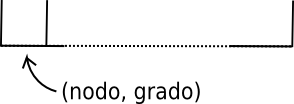
\includegraphics[height=1.5cm]{graficos/ejercicio4-1.png}
      \caption{vector gradosGrafo}
\end{figure}
\item Sabemos que el grafo solución va a tener la misma cantidad de nodos que G1 ya que el grafo formado por los nodos del grafo de menor tamaño sin aristas es un subgrafo de G2. Por lo tanto, lo que buscamos es agregarle la mayor cantidad de aristas que tengan en común los dos grafos iniciales.
\item Luego se tienen dos vectores, uno por cada grafo, donde se encuentran los nodos ordenados por grados. Ahora se mapea el nodo que se encuentra en la posición $i$ del vector correspondiente al grafo G1 con el nodo de la posición $i$ del grafo G2. Esto se hace para $i$ entre 0 y el tamaño del vector correspondiente a G1, es decir, entre 0 y la cantidad de nodos de G1. \\
\begin{figure}[H]
\centering
      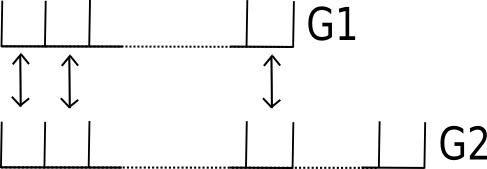
\includegraphics[height=2cm]{graficos/ejercicio4-2.png}
      \caption{Mapeo de grafos}
\end{figure}
\item Con este mapeo obtenido se calculan las aristas que tienen en común ambos grafos obteniendo así la solución al problema. 

\end{itemize}

\begin{algoritmo}{MCSgoloso}{\In{GrafoGrande}{vector(vector(int))}, \In{GrafoChico}{vector(vector(int))}, \In{gradosGrafoGrande}{vector(pair(int, int))}, \In{gradosGrafoGrande}{vector(pair(int, int))}}{vector(pair(int, int))}

	\For{(i = 0...gradosGrafoChico.size() - 1)}{
		mapeo[gradosGrafoChico[i].first] = gradosGrafoGrande[i].first; 
	}
	
	\tipo{vector(pair(int, int))} respuesta;
	respuesta = calcularConjAristas(mapeo, grafoChico, grafoGrande);
	return respuesta;      

\end{algoritmo}

\subsubsection*{Correctitud}
\noindent Veamos ahora que el resultado final es un subgrafo. Dado un mapeo válido se busca cuál es el conjunto de aristas que tienen en común ambos grafos renombrando cada nodo $i$ de G1 como $mapeo[i]$, es decir, el nodo que antes era el nodo $i$ ahora se llamará $mapeo[i]$.\\
Esto construye un subgrafo de ambos ya que para generar la respuesta se buscan las aristas que pertenecen a ambos grafos. 


\subsection{Complejidad}
Por claridad supondremos que el grafo G1 es el de menor cantidad de vértices (si son iguales, es indistinto).\\
El algoritmo implementado consta de 2 grandes etapas (aparte de las de recibir los datos y la de mostrarlos): la de ordenar por grados a los vértices, y la de mapear en orden y ver cuales son las aristas correspondientes que pueden ponerse en el mapeo.\\
Para la etapa de ordenar por grados, lo único que se hace es recorrer los grafos e ir guardando en un vector (uno por grafo) cada nodo con su grado (se tarda $\mathcal{O}(n_1+m_1)$ en recorrer el primero grafo y se tarda $\mathcal{O}(n_2+m_2)$ en recorrer el segundo). Luego se procede a ordenar por grado usando la función $sort(..)$ que, como esta especificado en la documentación de $C++$ (http://www.cplusplus.com/reference/algorithm/sort/), es $\mathcal{O}(n*log(n))$, con $n$ el tamaño el vector a ordenar. En particular, en este caso se tarda $\mathcal{O}(n_1*log(n_1)+n_2*log(n_2))$ en ordenar ambos vectores, que es igual a $\mathcal{O}(n_2*log(n_2))$ dado que asumimos a G2 el mas grande en cantidad de nodos.\\
En la segunda etapa, lo que se hace es mapear en el orden que quedaron luego de aplicar el sort y recorrer el grafo más chico (para este caso el G1) preguntando si por cada una de sus aristas, existe su equivalente en G2 luego de aplicar el mapeo. Recorrer las aristas de este G1 tiene complejidad $\mathcal{O}(n_1+m_1)$; para cada arista de este, se consulta en en su mapeo (la transformación del mapeo se realiza en $\mathcal{O}(1)$ pues es leer una posición determinada de un vector) los vecinos de el vértice de G2 correspondiente, esto (como sólo se recorren los vecinos de un único nodo ya determinado de G2) tarda $\mathcal{O}(m_2)$, por lo que en total la complejidad de esta etapa es $\mathcal{O}((n_1+m_1)*m_2)$.\\
Concluimos entonces que entre ambas etapas el orden de complejidad será la suma $\mathcal{O}((n_1+m_1)*m_2+n_2*log(n_2))$.


\subsection{Experimentación}
\noindent El algoritmo toma dos grafos para calcular el máximo subgrafo común, entonces para tomar las mediciones y determinar el tiempo de cómputo de la heurística, generalmente, se modificarán únicamente las cantidades de nodos y aristas de uno de ellos. \\
Sea $n_1$ y $m_1$ la cantidad de nodos y aristas del grafo que se modificará para tomar las mediciones respectivamente y $n_2$, $m_2$ la cantidad de nodos y aristas del grafo al que se le dejarán constantes las cantidades de nodos y aristas, aunque en cada caso podrán utilizarse grafos distintos por con la misma cantidad de vértices y de aristas.
    
	\subsubsection*{Experimento 1}\; 
\noindent  El objetivo de este experimento fue extraer conclusiones acerca de la variación en el tiempo de cómputo requerido por el algoritmo para distintos valores de $m_1$, con el fin de determinar su complejidad, dejando $n_1$ fijo. \\
   Para ello se utilizará un generador de grafos que funciona de la siguiente manera: dada una cantidad de vértices y aristas, en cada paso crea una nueva arista con extremos válidos (es decir, entre 0 y la cantidad de vértices - 1) y que no este repetida (que no haya sido creada todavía). 
   
     	\subsubsection*{Datos de entrada}\;
        \noindent Para correr el algoritmo con poda los valores de $m_1$ tomados fueron desde $0$ hasta $19900$ de $100$ en $100$. El valor de $n_1$ fue $200$.\\
       Los valores de $n_2$ y $m_2$ fueron $200$ y $2500$ respectivamente. Estos valores fueron elegidos de forma arbitraria.\\
        Para generar los grafos de forma aleatoria se utilizó el generador-grafo-rapido.cpp que se encuentra en la carpeta src y para correrlo se utilizó el exp1.sh que se encuentra en la carpeta exp/ejercicio4/exp1. \\
        Con el fin de acercarse a los valores reales y descartar posibles falsos resultados, se ejecuta la resolución del problema para cada una de los valores de $m_1$ siete veces considerando luego el promedio entre los valores obtenidos pero graficando también el desvío estándar (la cantidad de repeticiones a realizar fue elegida arbitrariamente).\; 
        \subsubsection*{Resultados}\;

    \begin{figure}[H]
      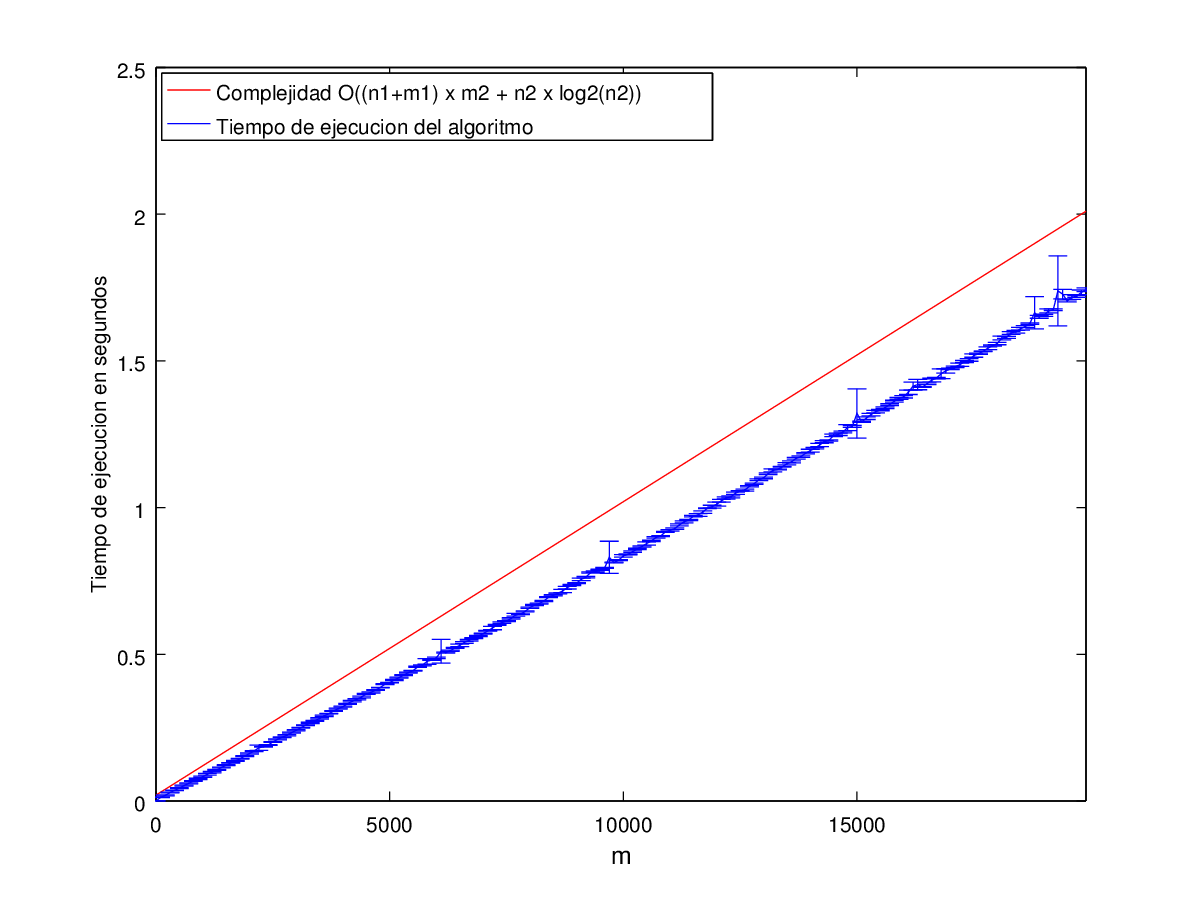
\includegraphics[height=10cm]{graficos/ejercicio4-exp1.png}
       \caption{Experimento 1}
	\end{figure}
        
\subsubsection*{Conclusiones}\;
Se concluye de observar el gráfico que se cumple la complejidad esperada para este caso en el que se mantiene la cantidad de nodos y se varía la cantidad de aristas, pues los tiempos de ejecución se mantienen por debajo de la línea de complejidad predicha.
    
    \subsubsection*{Experimento 2}\; 
    \noindent Este experimento es similar al anterior, pero ahora se varía la cantidad de nodos. Para ello, para cada cantidad de nodos se definirá una función para determinar la cantidad de aristas que tendrá el grafo. \\
    Se tuvieron en cuenta 4 funciones, con el fin de que el grafo obtenido no sea siempre uno especial y de esta forma poder analizar diferentes casos. 
        \begin{itemize}
        \item F1($n_1$) = $n_1$($n_1$-1))/2 = $m_1$ 
        \item F2($n_1$) = $n_1$-1 = $m_1$ 
        \item F3($n_1$) = 3$n_1$ = $m_1$
        \item F4($n_1$) = $n_1^{2}$/10 = $m_1$
		\end{itemize} 
 Para generar los grafos con estas cantidades de aristas y nodos se utilizó el mismo generador que en el experimento anterior.       
        
        
        \subsubsection*{Datos de entrada}\;
        
        \noindent Los valores de $n_1$ tomados fueron desde $100$ hasta $320$ de $20$ en $20$. \\
       Los valores de $n_2$ y $m_2$ fueron $320$ y $2500$ respectivamente. Estos valores fueron elegidos de forma arbitraria.\\
        Para generar los grafos de forma aleatoria se utilizó el generador-grafo-rapido.cpp que se encuentra en la carpeta src y para correrlo se utilizó el exp2.sh que se encuentra en la carpeta exp/ejercicio4/exp2. \\
        Con el fin de acercarse a los valores reales y descartar posibles falsos resultados, se ejecuta la resolución del problema para cada una de los valores de $n_1$ cinco veces considerando luego el promedio entre los valores obtenidos pero graficando también el desvío estándar (la cantidad de repeticiones a realizar fue elegida arbitrariamente).\; 
        
         \subsubsection*{Resultados}\;

    \begin{figure}[H]
      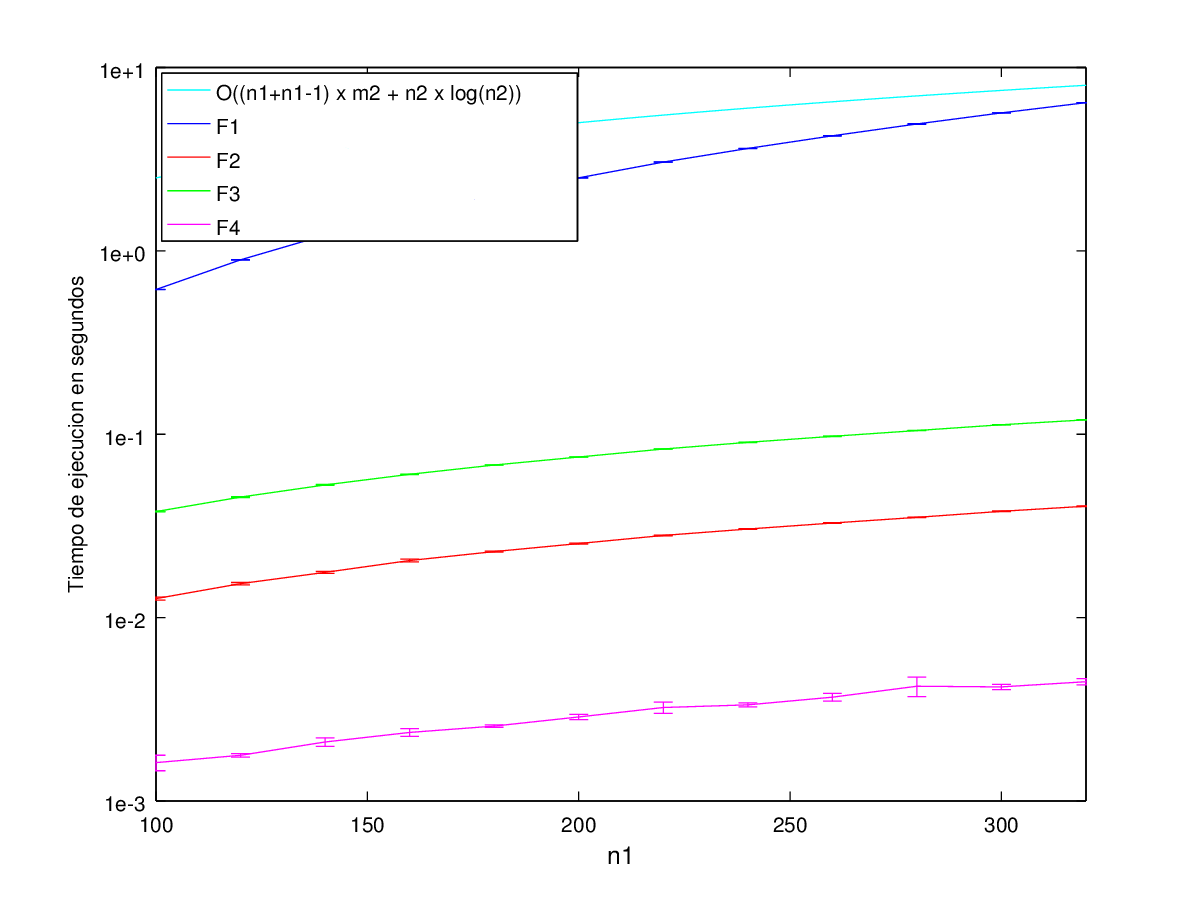
\includegraphics[height=10cm]{graficos/ejercicio4-exp2.png}
       \caption{Experimento 2}
	\end{figure}
        
     	\subsubsection*{Conclusiones}\;
En el gráfico se observa como todas las funciones de tiempo están por debajo de la curva de complejidad asintótica calculada. Se puede ver también como la diferencia en la cantidad de aristas influye en el tiempo de cómputo aunque siempre manteniéndose por debajo de la complejidad asintótica predicha.\\
Concluimos entonces que variando la cantidad de nodos, el tiempo de ejecución se mantendrá en el orden de complejidad predicho independientemente de la cantidad de aristas.
    
    \subsubsection*{Experimento 3}\; 
    El objetivo de este experimento fue extraer conclusiones acerca de la variación en el tiempo de cómputo requerido por el algoritmo para distintos valores de $m$ y $n$ variando los dos grafos al mismo tiempo pero siempre manteniendo $n_1$ igual a $n_2$ y $m_1$ igual a $m_2$. \\
Para generar los grafos con estas cantidades de aristas y nodos se utilizó el mismo generador que en el experimento anterior. 
        
        \subsubsection*{Datos de entrada}\;
        \noindent Los valores de $n$ tomados fueron desde $100$ hasta $1200$. Para cada $n$ se utilizó $3 \times n$ como cantidad de aristas.\\
        Para generar los grafos de forma aleatoria se utilizó el generador-grafo-rapido.cpp que se encuentra en la carpeta src y para correrlo se utilizó el exp3.sh que se encuentra en la carpeta exp/ejercicio4/exp3. \\
        Con el fin de acercarse a los valores reales y descartar posibles falsos resultados, se ejecuta la resolución del problema para cada una de los valores de $n$ cinco veces considerando luego el promedio entre los valores obtenidos pero graficando también el desvío estándar (la cantidad de repeticiones a realizar fue elegida arbitrariamente).\; 
 		\subsubsection*{Resultados}\;

    \begin{figure}[H]
      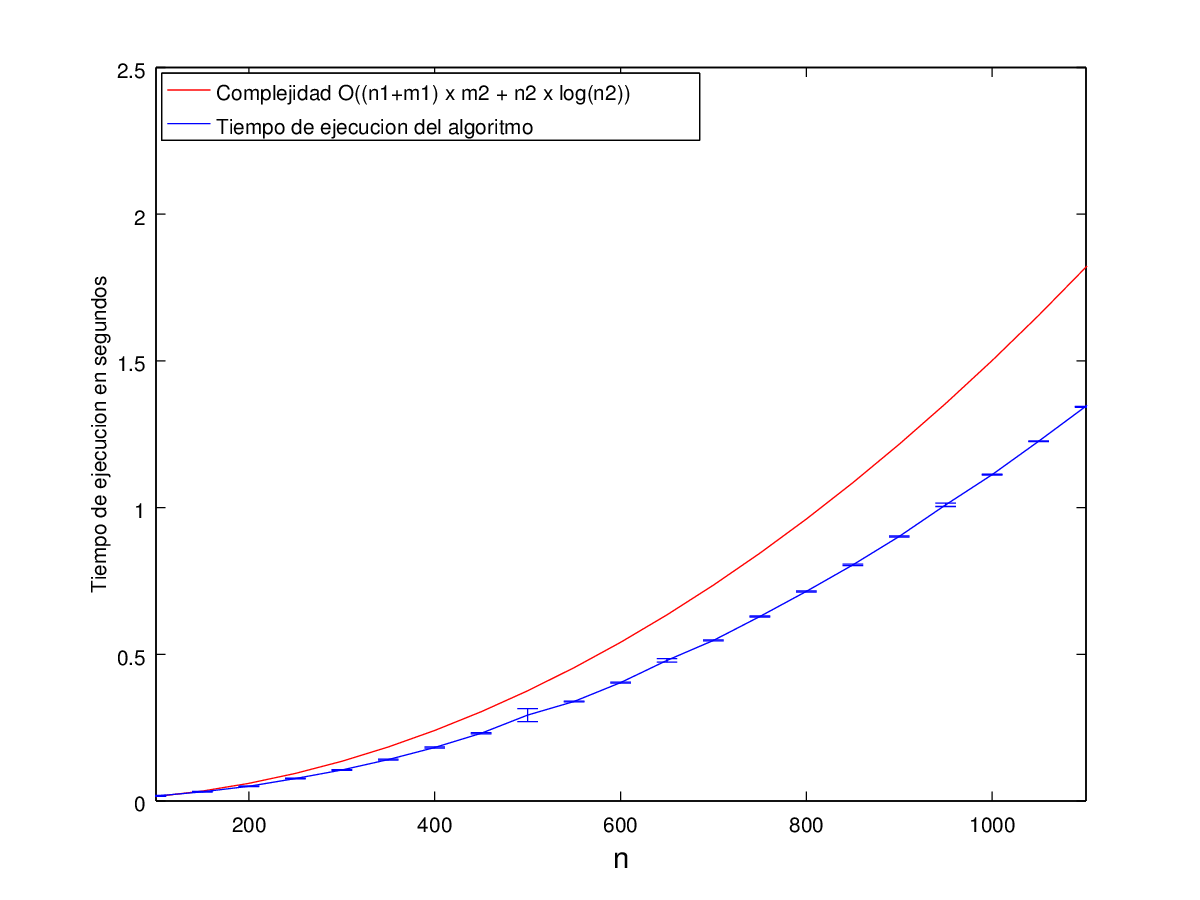
\includegraphics[height=10cm]{graficos/ejercicio4-exp3.png}
       \caption{Experimento 3}
	\end{figure}
        
     	\subsubsection*{Conclusiones}\;
Observamos en el gráfico que el comportamiento es el esperado, es decir que el tiempo de ejecución se mantiene por debajo del la complejidad temporal propuesta variando el $n_1=n_2$ y $m_1=m_2$.\\
    Concluimos que el algoritmo cumple con la complejidad propuesta anteriormente.